%\documentclass{standalone}
%\usepackage{tikz}
%\usetikzlibrary{patterns,plotmarks}
%\begin{document}
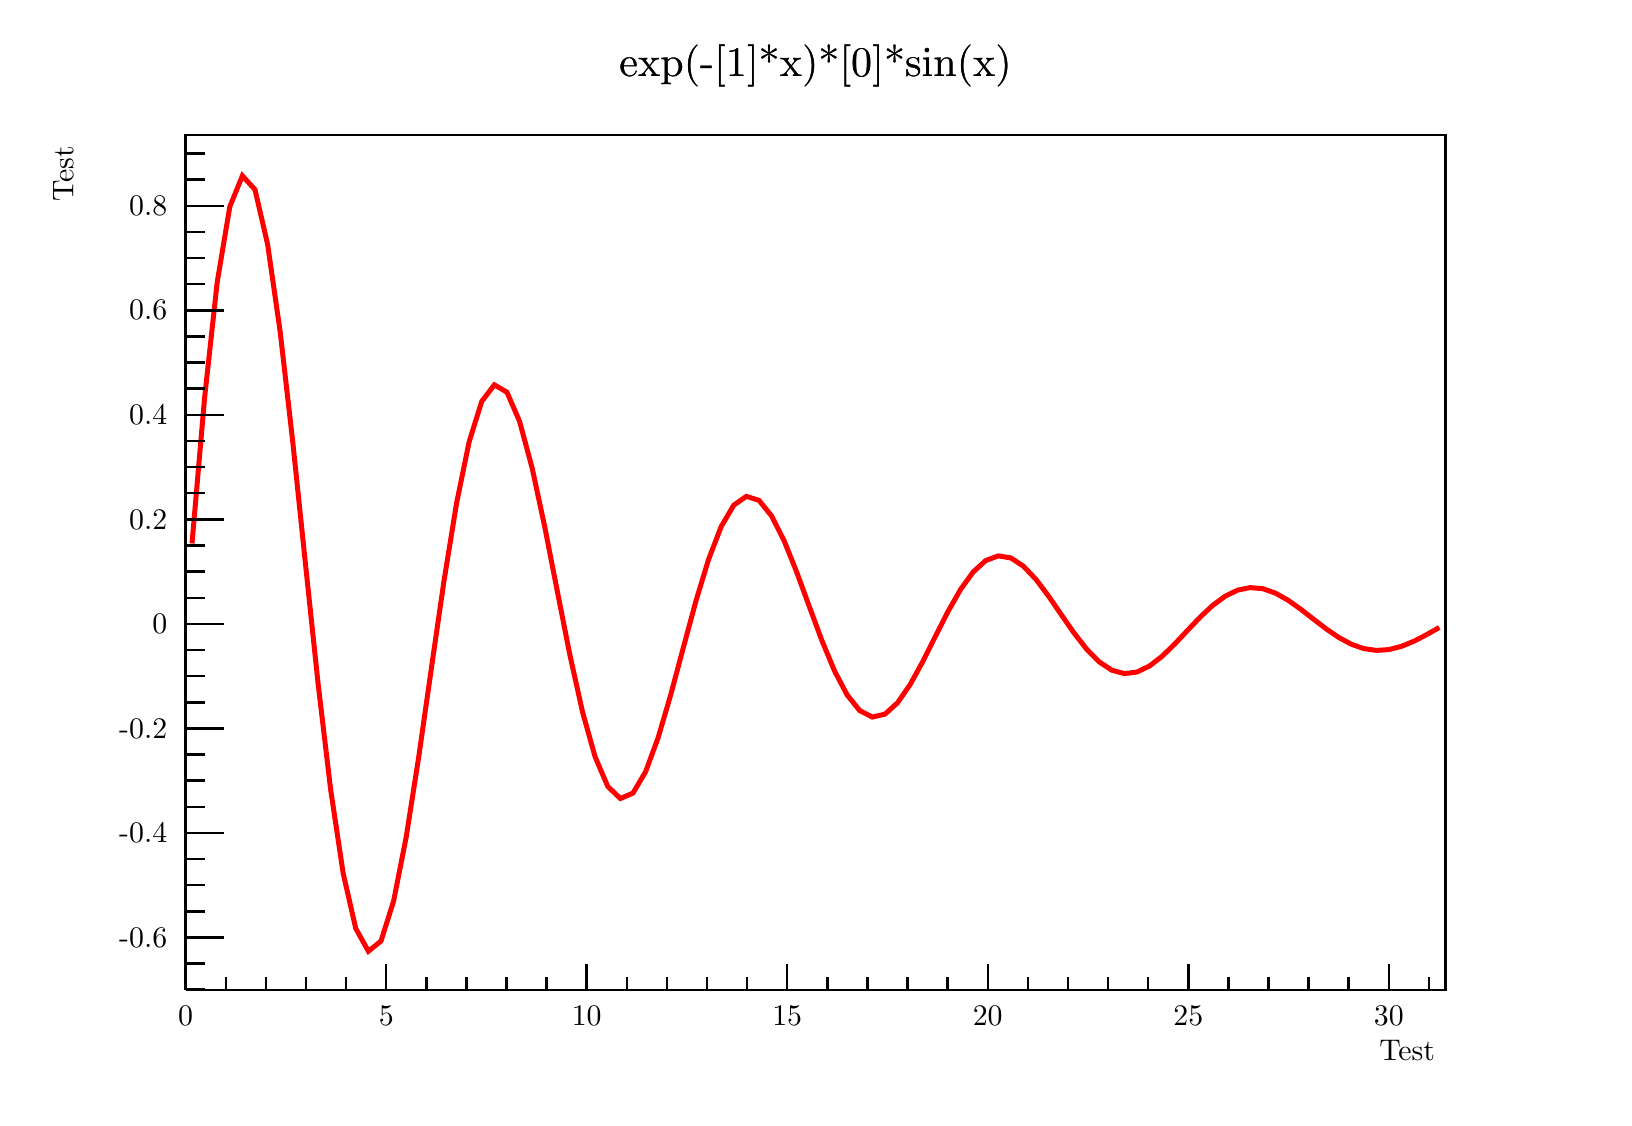
\begin{tikzpicture}
\def\CheckTikzLibraryLoaded#1{ \ifcsname tikz@library@#1@loaded\endcsname \else \PackageWarning{tikz}{usetikzlibrary{#1} is missing in the preamble.} \fi }
\CheckTikzLibraryLoaded{patterns}
\CheckTikzLibraryLoaded{plotmarks}
\pgfdeclareplotmark{cross} {
\pgfpathmoveto{\pgfpoint{-0.3\pgfplotmarksize}{\pgfplotmarksize}}
\pgfpathlineto{\pgfpoint{+0.3\pgfplotmarksize}{\pgfplotmarksize}}
\pgfpathlineto{\pgfpoint{+0.3\pgfplotmarksize}{0.3\pgfplotmarksize}}
\pgfpathlineto{\pgfpoint{+1\pgfplotmarksize}{0.3\pgfplotmarksize}}
\pgfpathlineto{\pgfpoint{+1\pgfplotmarksize}{-0.3\pgfplotmarksize}}
\pgfpathlineto{\pgfpoint{+0.3\pgfplotmarksize}{-0.3\pgfplotmarksize}}
\pgfpathlineto{\pgfpoint{+0.3\pgfplotmarksize}{-1.\pgfplotmarksize}}
\pgfpathlineto{\pgfpoint{-0.3\pgfplotmarksize}{-1.\pgfplotmarksize}}
\pgfpathlineto{\pgfpoint{-0.3\pgfplotmarksize}{-0.3\pgfplotmarksize}}
\pgfpathlineto{\pgfpoint{-1.\pgfplotmarksize}{-0.3\pgfplotmarksize}}
\pgfpathlineto{\pgfpoint{-1.\pgfplotmarksize}{0.3\pgfplotmarksize}}
\pgfpathlineto{\pgfpoint{-0.3\pgfplotmarksize}{0.3\pgfplotmarksize}}
\pgfpathclose
\pgfusepathqstroke
}
\pgfdeclareplotmark{cross*} {
\pgfpathmoveto{\pgfpoint{-0.3\pgfplotmarksize}{\pgfplotmarksize}}
\pgfpathlineto{\pgfpoint{+0.3\pgfplotmarksize}{\pgfplotmarksize}}
\pgfpathlineto{\pgfpoint{+0.3\pgfplotmarksize}{0.3\pgfplotmarksize}}
\pgfpathlineto{\pgfpoint{+1\pgfplotmarksize}{0.3\pgfplotmarksize}}
\pgfpathlineto{\pgfpoint{+1\pgfplotmarksize}{-0.3\pgfplotmarksize}}
\pgfpathlineto{\pgfpoint{+0.3\pgfplotmarksize}{-0.3\pgfplotmarksize}}
\pgfpathlineto{\pgfpoint{+0.3\pgfplotmarksize}{-1.\pgfplotmarksize}}
\pgfpathlineto{\pgfpoint{-0.3\pgfplotmarksize}{-1.\pgfplotmarksize}}
\pgfpathlineto{\pgfpoint{-0.3\pgfplotmarksize}{-0.3\pgfplotmarksize}}
\pgfpathlineto{\pgfpoint{-1.\pgfplotmarksize}{-0.3\pgfplotmarksize}}
\pgfpathlineto{\pgfpoint{-1.\pgfplotmarksize}{0.3\pgfplotmarksize}}
\pgfpathlineto{\pgfpoint{-0.3\pgfplotmarksize}{0.3\pgfplotmarksize}}
\pgfpathclose
\pgfusepathqfillstroke
}
\pgfdeclareplotmark{newstar} {
\pgfpathmoveto{\pgfqpoint{0pt}{\pgfplotmarksize}}
\pgfpathlineto{\pgfqpointpolar{44}{0.5\pgfplotmarksize}}
\pgfpathlineto{\pgfqpointpolar{18}{\pgfplotmarksize}}
\pgfpathlineto{\pgfqpointpolar{-20}{0.5\pgfplotmarksize}}
\pgfpathlineto{\pgfqpointpolar{-54}{\pgfplotmarksize}}
\pgfpathlineto{\pgfqpointpolar{-90}{0.5\pgfplotmarksize}}
\pgfpathlineto{\pgfqpointpolar{234}{\pgfplotmarksize}}
\pgfpathlineto{\pgfqpointpolar{198}{0.5\pgfplotmarksize}}
\pgfpathlineto{\pgfqpointpolar{162}{\pgfplotmarksize}}
\pgfpathlineto{\pgfqpointpolar{134}{0.5\pgfplotmarksize}}
\pgfpathclose
\pgfusepathqstroke
}
\pgfdeclareplotmark{newstar*} {
\pgfpathmoveto{\pgfqpoint{0pt}{\pgfplotmarksize}}
\pgfpathlineto{\pgfqpointpolar{44}{0.5\pgfplotmarksize}}
\pgfpathlineto{\pgfqpointpolar{18}{\pgfplotmarksize}}
\pgfpathlineto{\pgfqpointpolar{-20}{0.5\pgfplotmarksize}}
\pgfpathlineto{\pgfqpointpolar{-54}{\pgfplotmarksize}}
\pgfpathlineto{\pgfqpointpolar{-90}{0.5\pgfplotmarksize}}
\pgfpathlineto{\pgfqpointpolar{234}{\pgfplotmarksize}}
\pgfpathlineto{\pgfqpointpolar{198}{0.5\pgfplotmarksize}}
\pgfpathlineto{\pgfqpointpolar{162}{\pgfplotmarksize}}
\pgfpathlineto{\pgfqpointpolar{134}{0.5\pgfplotmarksize}}
\pgfpathclose
\pgfusepathqfillstroke
}
\definecolor{c}{rgb}{1,1,1};
\draw [color=c, fill=c] (0,0) rectangle (20,13.5714);
\draw [color=c, fill=c] (2,1.35714) rectangle (18,12.2143);
\definecolor{c}{rgb}{0,0,0};
\draw [c,line width=0.9] (2,1.35714) -- (2,12.2143) -- (18,12.2143) -- (18,1.35714) -- (2,1.35714);
\definecolor{c}{rgb}{1,0,0};
\draw [c,line width=1.8] (2.08,7.02833) -- (2.24,8.88067) -- (2.4,10.3448) -- (2.56,11.3041) -- (2.72,11.6973) -- (2.88,11.5213) -- (3.04,10.8276) -- (3.2,9.71412) -- (3.36,8.31323) -- (3.52,6.77661) -- (3.68,5.25975) -- (3.84,3.90679) -- (4,2.83739)
 -- (4.16,2.13675) -- (4.32,1.84953) -- (4.48,1.97809) -- (4.64,2.48478) -- (4.8,3.29803) -- (4.96,4.32125) -- (5.12,5.4436) -- (5.28,6.55152) -- (5.44,7.53972) -- (5.6,8.32082) -- (5.76,8.83257) -- (5.92,9.04235) -- (6.08,8.94845) -- (6.24,8.57836)
 -- (6.4,7.98436) -- (6.56,7.237) -- (6.72,6.41723) -- (6.88,5.60801) -- (7.04,4.88622) -- (7.2,4.31571) -- (7.36,3.94192) -- (7.52,3.7887) -- (7.68,3.85728) -- (7.84,4.12759) -- (8,4.56145) -- (8.16,5.10733) -- (8.32,5.70609) -- (8.48,6.29715) --
 (8.64,6.82435) -- (8.8,7.24105) -- (8.96,7.51406) -- (9.12,7.62598) -- (9.28,7.57589) -- (9.44,7.37845) -- (9.6,7.06156) -- (9.76,6.66285) -- (9.92,6.22551);
\draw [c,line width=1.8] (9.92,6.22551) -- (10.08,5.7938) -- (10.24,5.40873) -- (10.4,5.10437) -- (10.56,4.90496) -- (10.72,4.82322) -- (10.88,4.85981) -- (11.04,5.00402) -- (11.2,5.23547) -- (11.36,5.52669) -- (11.52,5.84613) -- (11.68,6.16145) --
 (11.84,6.4427) -- (12,6.66501) -- (12.16,6.81066) -- (12.32,6.87036) -- (12.48,6.84364) -- (12.64,6.73831) -- (12.8,6.56925) -- (12.96,6.35654) -- (13.12,6.12323) -- (13.28,5.89292) -- (13.44,5.68749) -- (13.6,5.52512) -- (13.76,5.41873) --
 (13.92,5.37512) -- (14.08,5.39464) -- (14.24,5.47158) -- (14.4,5.59506) -- (14.56,5.75042) -- (14.72,5.92083) -- (14.88,6.08905) -- (15.04,6.2391) -- (15.2,6.3577) -- (15.36,6.4354) -- (15.52,6.46725) -- (15.68,6.45299) -- (15.84,6.3968) --
 (16,6.30661) -- (16.16,6.19313) -- (16.32,6.06866) -- (16.48,5.94579) -- (16.64,5.8362) -- (16.8,5.74958) -- (16.96,5.69282) -- (17.12,5.66956) -- (17.28,5.67997) -- (17.44,5.72101) -- (17.6,5.78689) -- (17.76,5.86977);
\draw [c,line width=1.8] (17.76,5.86977) -- (17.92,5.96069);
\definecolor{c}{rgb}{0,0,0};
\draw [c,line width=0.9] (2,1.35714) -- (18,1.35714);
\draw [c,line width=0.9] (2,1.68286) -- (2,1.35714);
\draw [c,line width=0.9] (2.5093,1.52) -- (2.5093,1.35714);
\draw [c,line width=0.9] (3.01859,1.52) -- (3.01859,1.35714);
\draw [c,line width=0.9] (3.52789,1.52) -- (3.52789,1.35714);
\draw [c,line width=0.9] (4.03718,1.52) -- (4.03718,1.35714);
\draw [c,line width=0.9] (4.54648,1.68286) -- (4.54648,1.35714);
\draw [c,line width=0.9] (5.05578,1.52) -- (5.05578,1.35714);
\draw [c,line width=0.9] (5.56507,1.52) -- (5.56507,1.35714);
\draw [c,line width=0.9] (6.07437,1.52) -- (6.07437,1.35714);
\draw [c,line width=0.9] (6.58366,1.52) -- (6.58366,1.35714);
\draw [c,line width=0.9] (7.09296,1.68286) -- (7.09296,1.35714);
\draw [c,line width=0.9] (7.60225,1.52) -- (7.60225,1.35714);
\draw [c,line width=0.9] (8.11155,1.52) -- (8.11155,1.35714);
\draw [c,line width=0.9] (8.62085,1.52) -- (8.62085,1.35714);
\draw [c,line width=0.9] (9.13014,1.52) -- (9.13014,1.35714);
\draw [c,line width=0.9] (9.63944,1.68286) -- (9.63944,1.35714);
\draw [c,line width=0.9] (10.1487,1.52) -- (10.1487,1.35714);
\draw [c,line width=0.9] (10.658,1.52) -- (10.658,1.35714);
\draw [c,line width=0.9] (11.1673,1.52) -- (11.1673,1.35714);
\draw [c,line width=0.9] (11.6766,1.52) -- (11.6766,1.35714);
\draw [c,line width=0.9] (12.1859,1.68286) -- (12.1859,1.35714);
\draw [c,line width=0.9] (12.6952,1.52) -- (12.6952,1.35714);
\draw [c,line width=0.9] (13.2045,1.52) -- (13.2045,1.35714);
\draw [c,line width=0.9] (13.7138,1.52) -- (13.7138,1.35714);
\draw [c,line width=0.9] (14.2231,1.52) -- (14.2231,1.35714);
\draw [c,line width=0.9] (14.7324,1.68286) -- (14.7324,1.35714);
\draw [c,line width=0.9] (15.2417,1.52) -- (15.2417,1.35714);
\draw [c,line width=0.9] (15.751,1.52) -- (15.751,1.35714);
\draw [c,line width=0.9] (16.2603,1.52) -- (16.2603,1.35714);
\draw [c,line width=0.9] (16.7696,1.52) -- (16.7696,1.35714);
\draw [c,line width=0.9] (17.2789,1.68286) -- (17.2789,1.35714);
\draw [c,line width=0.9] (17.2789,1.68286) -- (17.2789,1.35714);
\draw [c,line width=0.9] (17.7882,1.52) -- (17.7882,1.35714);
\draw [anchor=base] (2,0.909286) node[scale=1.07876, color=c, rotate=0]{0};
\draw [anchor=base] (4.54648,0.909286) node[scale=1.07876, color=c, rotate=0]{5};
\draw [anchor=base] (7.09296,0.909286) node[scale=1.07876, color=c, rotate=0]{10};
\draw [anchor=base] (9.63944,0.909286) node[scale=1.07876, color=c, rotate=0]{15};
\draw [anchor=base] (12.1859,0.909286) node[scale=1.07876, color=c, rotate=0]{20};
\draw [anchor=base] (14.7324,0.909286) node[scale=1.07876, color=c, rotate=0]{25};
\draw [anchor=base] (17.2789,0.909286) node[scale=1.07876, color=c, rotate=0]{30};
\draw [anchor= east] (18,0.597143) node[scale=1.07876, color=c, rotate=0]{Test};
\draw [c,line width=0.9] (2,1.35714) -- (2,12.2143);
\draw [c,line width=0.9] (2.48,2.02411) -- (2,2.02411);
\draw [c,line width=0.9] (2.24,2.35596) -- (2,2.35596);
\draw [c,line width=0.9] (2.24,2.6878) -- (2,2.6878);
\draw [c,line width=0.9] (2.24,3.01965) -- (2,3.01965);
\draw [c,line width=0.9] (2.48,3.35149) -- (2,3.35149);
\draw [c,line width=0.9] (2.24,3.68334) -- (2,3.68334);
\draw [c,line width=0.9] (2.24,4.01519) -- (2,4.01519);
\draw [c,line width=0.9] (2.24,4.34703) -- (2,4.34703);
\draw [c,line width=0.9] (2.48,4.67888) -- (2,4.67888);
\draw [c,line width=0.9] (2.24,5.01073) -- (2,5.01073);
\draw [c,line width=0.9] (2.24,5.34257) -- (2,5.34257);
\draw [c,line width=0.9] (2.24,5.67442) -- (2,5.67442);
\draw [c,line width=0.9] (2.48,6.00626) -- (2,6.00626);
\draw [c,line width=0.9] (2.24,6.33811) -- (2,6.33811);
\draw [c,line width=0.9] (2.24,6.66996) -- (2,6.66996);
\draw [c,line width=0.9] (2.24,7.0018) -- (2,7.0018);
\draw [c,line width=0.9] (2.48,7.33365) -- (2,7.33365);
\draw [c,line width=0.9] (2.24,7.66549) -- (2,7.66549);
\draw [c,line width=0.9] (2.24,7.99734) -- (2,7.99734);
\draw [c,line width=0.9] (2.24,8.32919) -- (2,8.32919);
\draw [c,line width=0.9] (2.48,8.66103) -- (2,8.66103);
\draw [c,line width=0.9] (2.24,8.99288) -- (2,8.99288);
\draw [c,line width=0.9] (2.24,9.32472) -- (2,9.32472);
\draw [c,line width=0.9] (2.24,9.65657) -- (2,9.65657);
\draw [c,line width=0.9] (2.48,9.98842) -- (2,9.98842);
\draw [c,line width=0.9] (2.24,10.3203) -- (2,10.3203);
\draw [c,line width=0.9] (2.24,10.6521) -- (2,10.6521);
\draw [c,line width=0.9] (2.24,10.984) -- (2,10.984);
\draw [c,line width=0.9] (2.48,11.3158) -- (2,11.3158);
\draw [c,line width=0.9] (2.48,2.02411) -- (2,2.02411);
\draw [c,line width=0.9] (2.24,1.69226) -- (2,1.69226);
\draw [c,line width=0.9] (2.24,1.36042) -- (2,1.36042);
\draw [c,line width=0.9] (2.48,11.3158) -- (2,11.3158);
\draw [c,line width=0.9] (2.24,11.6476) -- (2,11.6476);
\draw [c,line width=0.9] (2.24,11.9795) -- (2,11.9795);
\draw [anchor= east] (1.9,2.02411) node[scale=1.07876, color=c, rotate=0]{-0.6};
\draw [anchor= east] (1.9,3.35149) node[scale=1.07876, color=c, rotate=0]{-0.4};
\draw [anchor= east] (1.9,4.67888) node[scale=1.07876, color=c, rotate=0]{-0.2};
\draw [anchor= east] (1.9,6.00626) node[scale=1.07876, color=c, rotate=0]{0};
\draw [anchor= east] (1.9,7.33365) node[scale=1.07876, color=c, rotate=0]{0.2};
\draw [anchor= east] (1.9,8.66103) node[scale=1.07876, color=c, rotate=0]{0.4};
\draw [anchor= east] (1.9,9.98842) node[scale=1.07876, color=c, rotate=0]{0.6};
\draw [anchor= east] (1.9,11.3158) node[scale=1.07876, color=c, rotate=0]{0.8};
\draw [anchor= east] (0.442857,12.2143) node[scale=1.07876, color=c, rotate=90]{Test};
\draw (10,13.0921) node[scale=1.52295, color=c, rotate=0]{exp(-[1]*x)*[0]*sin(x)};
\draw (10,13.0921) node[scale=1.52295, color=c, rotate=0]{exp(-[1]*x)*[0]*sin(x)};
\end{tikzpicture}
%\end{document}
